%!TEX root = ../main.tex
%%%%%%%%%%%%%%%%%%%%%%%%%%%%%%%%%%
% Links:
%
% Difficulty:
% Companies: 
%%%%%%%%%%%%%%%%%%%%%%%%%%%%%%%%%%


%\begin{figure}
%	\centering
%	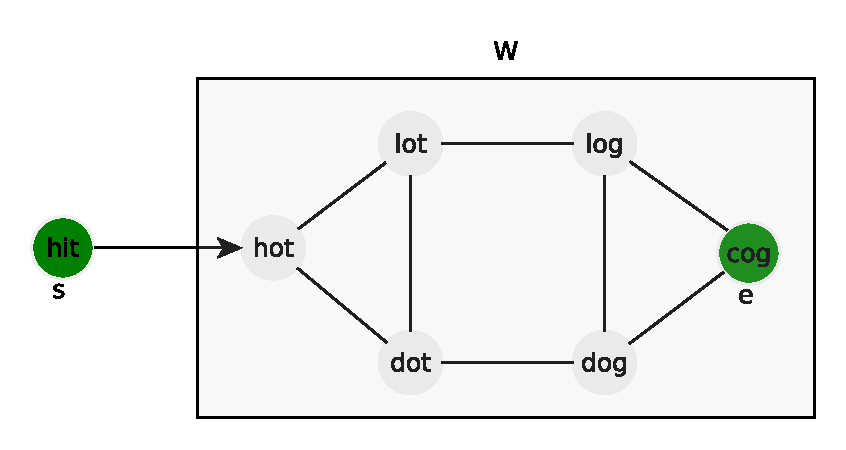
\includegraphics[width=\textwidth]{sources/word_ladder/images/example1}
%	\caption[Sample short cpation]{Sample Caption}.
%	\label{fig:word_ladder:example1}
%\end{figure}

\chapter{Word Ladder}
\label{ch:word_ladder}
\section*{Introduction}
\begin{wrapfigure}{r}{0.1\textwidth}
    \vspace{-30pt}
    \begin{center}
        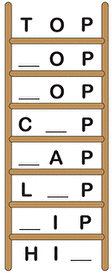
\includegraphics[scale=0.5]{sources/word_ladder/images/top-word-ladder}
    \end{center}
  \end{wrapfigure}
String is a popular topic in coding interivew and there are literally conuntless examplex of real-world interviews where strings are involved in some ways or another.
This manuscript already contains several string questions in chapters: \ref{ch:string_to_int} (page \pageref{ch:string_to_int}), \ref{ch:string_reverse} (page \pageref{ch:string_reverse}) and \ref{ch:two_string_anagram} (page \pageref{ch:two_string_anagram})).
Among this plethora of questions, \textit{word ladder} is definitely one of the most known and feared (at the time of writing it has one of the lowest acceptance rates on \href{https://leetcode.com/problems/word-ladder/}{leetcode.com}), as is considered a quite challenging and hard problem to solve during live coding interview. 
We feel however that its bad reputation is unjustified because, as we will see below, it can be approached by using known algorithmic tools and concepts when framed as a graph connectivity problem.


\section{Problem statement}
\begin{exercise}
\label{example:word_ladder:exercice1}
We are given two strings $s$ and $e$ and a list of strings $W=\{w_0, w_1,\ldots,w_{n-1}\}$ of size $n$.
Let a sequence $S=s_0 = s \rightarrow s_1 \rightarrow s_2 \rightarrow \ldots \rightarrow s_n = e$ be defined as a \textit{transformation} if and only if 
\begin{itemize}
	\item $s_i$ differs from from its adjecent neighboring strings in the sequence, $s_{i-1}$ and $s_{i+1}$, in exactly one character;
	\item each elements of the sequence, from second to last, is also in $W$ i.e. $s_i \in W \: \: 1 \leq n-1 $
\end{itemize}
Write a function that given $s,e$ and $W$ return the length of the smallest valid transformation.
If no transfromation exists the function should return $0$.

	%example1
	\begin{example}
		\label{example:word_ladder:example1}
		\hfill \\
		Given $s=$\textit{hit},  $e=$\textit{cog} and $W=\{$\textit{hot},\textit{dot},\textit{dog},\textit{lot},\textit{log},\textit{cog}$\}$, the function returns $5$.
		A possible valid transformation  of minimal length is: \textit{hit} $\rightarrow$ \textit{hot} $\rightarrow$ \textit{dot} $\rightarrow$ \textit{dog} $\rightarrow$ \textit{cog}.

		Notice that if for instance $e=$\textit{fog}, the the function would return $0$ as \textit{fog} $\notin W$.
	\end{example}

\end{exercise}

\section{Clarification Questions}

\begin{QandA}
	\item What is the maximum length of each word in $W$?
	\begin{answered}
		\textit{Up to $10$ characters.}
	\end{answered}
	
	\item Is it guaranteed for all input strings ($s$ and $e$ included) to be of the same length?
	\begin{answered}
		\textit{Yes}
	\end{answered}

	\item Are there duplicates in $W$?
	\begin{answered}
		\textit{No, you might assume $W$ to only contains unique words.}
	\end{answered}

	\item How many words are in $W$ at most?
	\begin{answered}
		\textit{Up to $2\times 10^4$.}
	\end{answered}

\end{QandA}

\section{Discussion}
\label{word_ladder:sec:discussion}


\subsection{BFS}
\label{word_ladder:sec:bruteforce}


\begin{figure}
	\centering
	\begin{subfigure}[]{0.95\textwidth}
		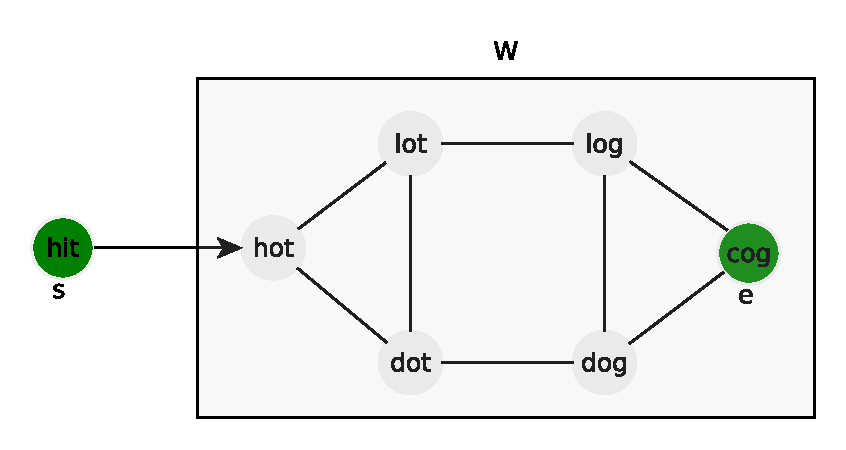
\includegraphics[width=\textwidth]{sources/word_ladder/images/example1}
		\caption[n]{Graph representation of Example \ref{example:word_ladder:example1}.}
		\label{fig:word_ladder:example1}
	 \end{subfigure}
	\hfill
	\begin{subfigure}[]{1.17\textwidth}
		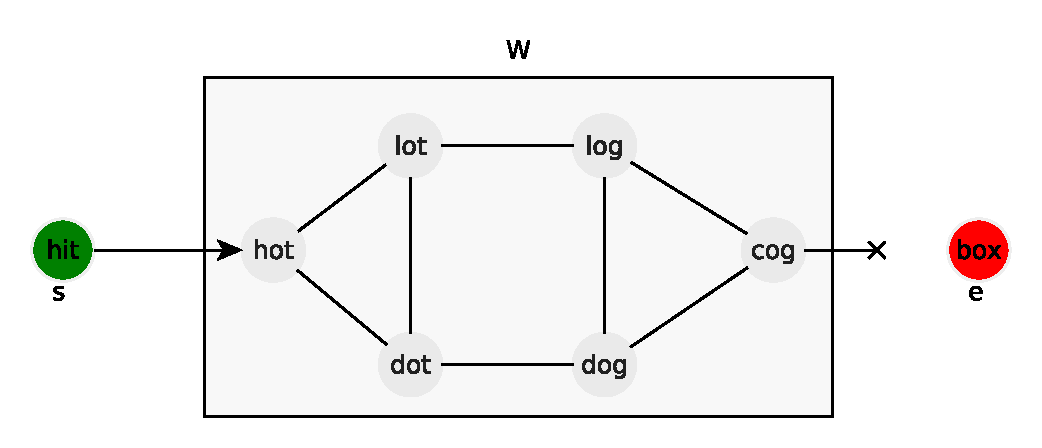
\includegraphics[width=\textwidth]{sources/word_ladder/images/example2}
		\caption[n]{Graph representation of Example \ref{example:word_ladder:example1} when $e=$\textit{box}. Notice how node \textit{box} is disconnected from the component containing \textit{hit}.}
		\label{fig:word_ladder:example1}
	\end{subfigure}
\end{figure}
    


\begin{minipage}{\linewidth}
	\lstinputlisting[language=c++, caption={Sample Caption},label=list:word_ladder]{sources/word_ladder/word_ladder_solution1.cpp}
\end{minipage}

